\lecture{10}{Wed 24 Jan '24}{}

\begin{theorem}[Multinomial theorem] \label{thm:multinomial}
    Let $n, k \in \N$ and $x_1, \dots, x_k$ be indeterminates.
    Then \[
        \sum_{\substack{0\le a_1, \dots, a_k \le n \\ a_1 + \dots + a_k = n}}
        \binom{n}{a_1, \dots, a_k} x_1^{a_1} \dots x_k^{a_k} = (x_1 + \dots + x_k)^n
    \]
\end{theorem}
\begin{proof}
    % TODO: bijection between terms on left and right
\end{proof}

\begin{example}
    \begin{align*}
        \binom{1/2}{n}
            &= \frac{(1/2)(-1/2) \dots (1/2 - n + 1)}{n} \\
            &= \frac{(-1)^{n - 1} (2n - 3)!!}{2^n n!}
    \end{align*}
\end{example}

\begin{definition} \label{def:composition}
    A \emph{weak composition} of $n \in \N$ is a sequence $(a_i)_{i=1}^k$
    where $a_i \in \N$ and $a_1 + \dots + a_k = n$.
    If each $a_i > 0$, then it is called a \emph{(strict) composition}.
\end{definition}
\begin{example}
    For $n = 3$, its strict compositions are $(1, 1, 1)$, $(1, 2)$, $(2, 1)$
    and $(3)$.
\end{example}

\begin{proposition} \label{thm:composition:count}
    The number of weak compositions of $n$ into $k$ parts is
    $\binom{n+k-1}{k-1}$.
\end{proposition}
\begin{proof}
    % TODO: bijection with $n$ balls in $k$ boxes.
\end{proof}
\begin{corollary}
    The number of compositions of $n$ into $k$ parts is $\binom{n-1}{k-1}$.
\end{corollary}
\begin{proof}
    Each box must get at least one ball, so use \cref{thm:composition:count}
    with $n \mapsto n - k$.
\end{proof}
\begin{corollary}
    The total number of compositions is $2^{n-1}$.
\end{corollary}
\begin{proof}
    $\sum_{k=1}^{n} \binom{n-1}{k-1} = \sum_{k=0}^{n-1} \binom{n-1}{k}
    = 2^{n-1}$.
\end{proof}

\begin{definition}[Partitions] \label{def:partitions}
    An \emph{(integer) partition} of $n \in \N$ is a sequence
    $\lambda = (\lambda_1, \dots, \lambda_k)$ of weakly decreasing positive
    integers which sum to $n$.
    We write $\lambda \vdash n$.
    Each $\lambda_i$ is called a \emph{part} and the number of parts is
    called the \emph{length}, denoted $\ell(\lambda)$.
    We write $p(n)$ for the number of partitions of $n$.
\end{definition}
\begin{example}
    The partitions of $5$ are $(5)$, $(4, 1)$, $(3, 2)$, $(3, 1, 1)$,
    $(2, 2, 1)$, $(2, 1, 1, 1)$ and $(1, 1, 1, 1, 1)$.
    Thus $p(5) = 7$.
\end{example}

\begin{proposition} \label{thm:partitions:conj}
    The number of partitions of $n$ into exactly (resp. at most) $k$ parts
    is the same as the number of partitions of $n$ with largest part exactly
    (resp. at most) $k$.
\end{proposition}

\begin{definition} \label{def:young}
    The \emph{Young/Ferrers diagram} of a partition is a left-justified
    array of boxes with $\lambda_i$ boxes in the $i$th row.
\end{definition}
\begin{example}
    The Young diagrams of $(4, 1)$ and $(3, 2)$ are
    \begin{center}
        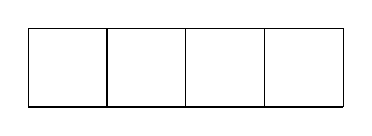
\begin{tikzpicture}
            \draw (0, 0) grid (4, 1);
        \end{tikzpicture}
        \qquad
        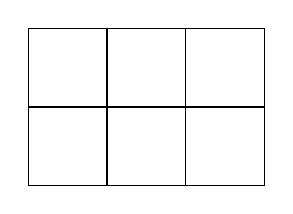
\begin{tikzpicture}
            \draw (0, 0) grid (3, 2);
        \end{tikzpicture}
    \end{center}
\end{example}

\begin{definition}[Conjugate] \label{def:partition:conjugate}
    The \emph{conjugate} of a partition $\lambda$, denoted $\lambda'$, is
    the partition whose Young diagram is the transpose of that of $\lambda$.
    That is, \[
        \lambda'_i = \size \set{j \in \N : \lambda_j \ge i}
    \]
\end{definition}

\begin{proof}[Proof of \cref{thm:partitions:conj}]
    If $\lambda$ has length $k$, then $\lambda'$ has largest part $k$.
\end{proof}

\begin{theorem}
    The number of self-conjugate partitions of $n$ is equal to the number
    of partitions of $n$ into distinct odd parts.
\end{theorem}
\begin{proof}
    % TODO
\end{proof}

\begin{theorem}[Euler] \label{thm:partitions:euler}
    The number of partitions of $n$ into odd parts is equal to the number
    of partitions of $n$ into distinct parts.
\end{theorem}

\begin{fact}[Hardy-Ramanujan Formula] \label{thm:partitions:ramanujan}
    \[
        p(n) \sim \frac{1}{4n\sqrt{3}} e^{\pi \sqrt{\frac{2n}{3}}}
    \]
\end{fact}

\begin{definition} \label{def:set_partitions}
    A \emph{set partition} of $[n]$ is a collection of pairwise disjoint
    non-empty subsets/blocks whose union is $[n]$.
    The number of set partitions of $[n]$ into $k$ (non-empty) blocks is
    called the \emph{Stirling number of the second kind} and denoted
    $\stirling{n}{k}$, read ``$n$ set $k$''.
\end{definition}
\begin{example}
    The set partitions of $[3]$ are $123$, $12|3$, $13|2$, $1|23$ and
    $1|2|3$.
\end{example}
